\title{\textbf{FASA: Frequency/Variance-Aware Sparse Attention for Bidirectional Encoders}}

\author{Anonymous authors}



\section{Introduction}

\subsection{Motivation}

The quadratic cost of attention is dominated by the product $QK^\top$ and 
the subsequent multiplication $AV$. Both scale with the number of key/value 
tokens. If we can reduce the effective number of KV tokens from $L$ to 
$L' < L$, both operations scale down: $QK^\top$ becomes $O(L \cdot L')$ 
instead of $O(L^2)$, and $AV$ becomes $O(L \cdot L' \cdot d_h)$.

\textbf{Token pruning} methods exploit this by dropping a subset of KV tokens 
at inference time. The question is \textbf{which tokens to drop}.

0.85


\subsection{Problem Statement}

Given keys $K \in \mathbb{R}^{B \times H \times L \times d_h}$ and values 
$V \in \mathbb{R}^{B \times H \times L \times d_h}$, select a subset 
$\mathcal{S} \subset \{1, \ldots, L\}$ with $|\mathcal{S}| = r L$ such that:

\[
\text{Attn}(Q, K_{\mathcal{S}}, V_{\mathcal{S}}) \approx \text{Attn}(Q, K, V)
\tag{1.1}
\]

while computing the left-hand side at a fraction $r$ of the cost.

\subsection{Our Approach}

FASA ranks tokens by the mean-over-heads variance of their key vectors:

\[
\text{imp}_i = \frac{1}{H} \sum_{h=1}^{H} \text{Var}_d(K_{i,h,d})
\tag{1.2}
\]

and retains the top-$rL$ tokens. Index 0 (the CLS token) is always 
preserved, motivated by the attention-sink literature.

\textbf{Special cases:}
\begin{itemize}
\item \textbf{Causal decoders:} FASA does not prune. The causal code path uses full
  attention to preserve strict lower-triangular masking.
\item \textbf{Cross-attention:} FASA does not prune. Pruning would break the
  alignment between query and key positions.

\end{itemize}
\subsection{Contributions}

\begin{itemize}
\item \textbf{FASA}, a variance-based token pruning method with a fixed keep ratio.
\item \textbf{Bidirectional-only application.} We document that causal decoders
  cannot use FASA without breaking causality.
\item \textbf{Empirical evaluation} on DistilBERT, RoBERTa, and GPT-2 on SST-2.
\item \textbf{Full reproducibility}, including code and checkpoints.

\end{itemize}
\subsection{Paper Organization}

Section 2 reviews token pruning, KV cache compression, and attention sinks. 
Section 3 provides background on attention and variance. Section 4 presents 
FASA. Section 5 covers integration. Section 6 details the setup. Section 7 
reports results. Section 8 analyzes the pruning behavior. Section 9 
discusses. Section 10 lists limitations. Section 11 concludes.



\subsection{Notation}

\begin{table}[H]
\centering
\small
\begin{tabular}{lll}
\toprule
\textbf{Symbol} & \textbf{Meaning} & \textbf{First appears} \\
\midrule
$L$ & Sequence length & 1.1 \\
$d_h$ & Head dimension & 1.1 \\
$H$ & Number of heads & 1.2 \\
$r$ & Keep ratio & 1.3 \\
$\text{imp}_i$ & Importance score of token $i$ & 1.3 \\
$\mathcal{S}$ & Selected subset & 1.2 \\
\bottomrule
\end{tabular}
\end{table}
</parameter>
\begin{lstlisting}

---
\end{lstlisting}


\section{Related Work}

\subsection{Token Pruning and KV Compression}

\textbf{H2O} (Zhang et al., 2023). Keeps "heavy-hitter" tokens based on 
accumulated attention scores. Requires attention scores at each step, which 
FASA does not.

\textbf{StreamingLLM} (Xiao et al., 2024). Pins the first few tokens as attention 
sinks and keeps a sliding window. FASA's CLS-pinning is inspired by this.

\textbf{SnapKV} (Li et al., 2024). Uses attention scores from a prefix window to 
select which tokens to keep. FASA uses variance instead.

\textbf{Scissorhands} (Liu et al., 2023). Uses an importance criterion based on 
past attention patterns.

\textbf{PyramidKV} (Cai et al., 2024). Allocates different budgets to different 
layers.

\subsection{Attention Sinks}

\textbf{Xiao et al. (2024)} and \textbf{Gu et al. (2024)} show that transformers 
allocate disproportionate attention to the first few tokens. This is the 
basis for CLS-pinning in FASA.

\subsection{Sparse Attention}

\textbf{Longformer} (Beltagy et al., 2020). Sliding-window + global.

\textbf{BigBird} (Zaheer et al., 2020). Sliding-window + random + global.

\textbf{FASA differs from these} in that sparsity is \textbf{data-dependent} 
(variance of K) rather than architecturally fixed.

\subsection{Position of Our Work}

\begin{table}[H]
\centering
\small
\begin{tabular}{lll}
\toprule
\textbf{Axis} & \textbf{Prior work} & \textbf{FASA} \\
\midrule
\textbf{Importance criterion} & Attention scores (H2O, SnapKV) & \textbf{Variance of K} \\
\textbf{Sink pinning} & First few tokens & \textbf{CLS only} \\
\textbf{Causal support} & Yes (with careful masking) & \textbf{No (skips pruning)} \\
\textbf{Training required} & No & No \\
\textbf{Parameters added} & None & LoRA only \\
\bottomrule
\end{tabular}
\end{table}

\textbf{Key distinction.} FASA's importance criterion is \textbf{cheaper} than H2O 
(no attention scores needed) but is \textbf{weaker} as a signal. Our ablation 
in Section 8 quantifies this.



\subsection{Comparison Table}

\begin{lstlisting}

---
\end{lstlisting}


\section{Background}

\subsection{Scaled Dot-Product Attention}

\[
\text{Attn}(Q, K, V) = \text{softmax}\!\left(\frac{QK^\top}{\sqrt{d_h}}\right)V
\tag{3.1}
\]

\textbf{Cost analysis.} The score matrix $QK^\top$ is $O(B H L^2)$. The value 
matmul $AV$ is $O(B H L^2 d_h)$.

\subsection{Token Pruning}

Replace $K, V$ with subsets $K_{\mathcal{S}}, V_{\mathcal{S}}$:

\[
\text{Attn}'(Q, K, V) = \text{softmax}\!\left(\frac{QK_{\mathcal{S}}^\top}{\sqrt{d_h}}\right)V_{\mathcal{S}}
\tag{3.2}
\]

\textbf{Cost.} $O(B H L \cdot |\mathcal{S}|)$ for scores and $O(B H L |\mathcal{S}| d_h)$ 
for the value matmul. With $|\mathcal{S}| = rL$, cost reduces by factor $r$.

\subsection{Variance as Importance}

For a token's key vector $k \in \mathbb{R}^{d_h}$:

\[
\text{Var}(k) = \frac{1}{d_h} \sum_{j=1}^{d_h} (k_j - \bar{k})^2
\tag{3.3}
\]

\textbf{Intuition.} Tokens whose keys have high variance have distinctive 
dimensional activations. They are likely to be attended to because their 
key inner-products with queries will span a wider range.

\textbf{Counter-argument.} This is a \textbf{heuristic}. Tokens with low-variance 
keys may still be highly attended if all queries align with them. Conversely, 
high-variance keys may be noisy and unattended. The signal is imperfect.

\subsection{Attention Sinks}

\textbf{Empirical observation.} The first token receives disproportionate 
attention in most transformer layers, even without any specific pretraining 
objective targeting this.

\textbf{Consequence.} Pruning the first token is catastrophic. FASA protects it:

\begin{lstlisting}
importance[:, 0] = 1e9
\end{lstlisting}

\subsection{LoRA}

LoRA (Hu et al., 2021):

\[
W_{\text{eff}} = W_{\text{frozen}} + \frac{\alpha}{r_L} BA
\tag{3.4}
\]

Used for recovery after injection.

\subsection{Notation Summary}

\begin{table}[H]
\centering
\small
\begin{tabular}{ll}
\toprule
\textbf{Symbol} & \textbf{Meaning} \\
\midrule
$L$ & Sequence length \\
$d_h$ & Head dimension \\
$H$ & Number of heads \\
$r$ & Keep ratio \\
$\mathcal{S}$ & Selected token subset \\
$\text{Var}(k)$ & Variance of key vector \\
$r_L$ & LoRA rank \\
\bottomrule
\end{tabular}
\end{table}
</parameter>
\begin{lstlisting}

---
\end{lstlisting}


\section{Method}

\subsection{Overview}

FASA has two paths:

\begin{lstlisting}
                 Input X
                    |
                     
              +-----------+
              |  Q/K/V    |
              | projection|
              +-----+-----+
                    |
                     
              +-----------+
              | is_causal |
              | or cross? |
              +--+----+---+
                 | No | Yes
                 |    |
                       
       +----------+  +------------------+
       | FASA     |  | Standard full    |
       | prune    |  | attention        |
       | K/V      |  | (no pruning)     |
       +----+-----+  +----------+-------+
            |                   |
            +----+--------------+
                 |
                  
           Output Y
\end{lstlisting}

\subsection{Importance Scoring}

For keys $K \in \mathbb{R}^{B \times H \times L \times d_h}$:

\[
\text{imp}(b, i) = \frac{1}{H} \sum_{h=1}^{H} \text{Var}_{d_h}(K_{b,h,i,:})
\tag{4.1}
\]

\textbf{Two aggregation steps:}
\begin{enumerate}
\item \textbf{Variance over head dimension $d_h$.} For each (batch, head, position),
  compute the variance of the $d_h$-dimensional key vector.
\item \textbf{Mean over heads.} Aggregate across heads into a per-position score.

\end{enumerate}
\textbf{Default method:} \texttt{importance\_method = "var"}.

\textbf{Alternative:} \texttt{importance\_method = "l2"} uses the L2 norm of the key 
instead:

\[
\text{imp}(b, i) = \frac{1}{H} \sum_{h=1}^{H} \|K_{b,h,i,:}\|_2
\tag{4.2}
\]

\subsection{CLS Pinning}

Index 0 is always preserved:

\[
\text{imp}(b, 0) \leftarrow 10^9
\tag{4.3}
\]

This ensures CLS is selected by the top-$k$ operation regardless of its 
variance.

\subsection{Top-$k$ Selection}

Let $r$ be the keep ratio. The number of tokens to keep:

\[
k = \max\!\left(8, \min\!\left(L, \lfloor r L \rfloor\right)\right)
\tag{4.4}
\]

The \texttt{max(8, ...)} floor prevents over-pruning short sequences.

The selected indices:

\[
\mathcal{S} = \text{topk}_k(\text{imp}) \quad \text{(sorted ascending)}
\tag{4.5}
\]

Sorting ensures stable gather and preserves positional order.

\subsection{Pruned Attention}

Given $\mathcal{S}$, gather:

\[
K_{\mathcal{S}} = \text{gather}(K, \mathcal{S}), \quad
V_{\mathcal{S}} = \text{gather}(V, \mathcal{S})
\tag{4.6}
\]

Then compute standard attention:

\[
\text{Attn}' = \text{softmax}\!\left(\frac{Q K_{\mathcal{S}}^\top}{\sqrt{d_h}}\right)V_{\mathcal{S}}
\tag{4.7}
\]

\textbf{Cost reduction.} Scores matrix: $L \times L$ $\to$ $L \times k$. Value matmul: 
$L \times L \times d_h$ $\to$ $L \times k \times d_h$.

\subsection{The Decoder Path}

\textbf{Critical.} For causal attention, FASA \textbf{does not prune}. The code:

\begin{lstlisting}
is_causal = bool(self.is_decoder and not is_cross and L > 1)
if is_causal or is_cross:
    # Standard full attention
    scores = torch.matmul(q.float(), k.float().transpose(-2, -1)) * scale
    if is_causal:
        causal_mask = torch.triu(...)
        scores = scores + causal_mask
    ...
\end{lstlisting}

\textbf{Why?} Pruning would remove tokens from the middle of the sequence. For 
causal attention, a query at position $i$ attends to all $j \leq i$; if we 
prune some $j$, the causal mask's diagonal structure is broken. To preserve 
strict causality, FASA skips pruning.

\textbf{Consequence.} For GPT-2, FASA does \textbf{no sparsification} -- it acts as a 
LoRA-only adapter.

\subsection{Parameter Analysis}

\begin{table}[H]
\centering
\small
\begin{tabular}{lll}
\toprule
\textbf{Component} & \textbf{Baseline} & \textbf{FASA} \\
\midrule
Q/K/V/O projections & $4d^2$ & $4d^2 + \text{LoRA}$ \\
Other & 0 & 0 \\
\bottomrule
\end{tabular}
\end{table}

\textbf{FASA does not add non-LoRA parameters.} The pruning is purely 
algorithmic.

\subsection{Complexity Analysis}

\begin{table}[H]
\centering
\small
\begin{tabular}{lll}
\toprule
\textbf{Path} & \textbf{Time} & \textbf{Memory} \\
\midrule
Bidirectional (pruned) & $O(L \cdot k \cdot d_h + L d^2)$ & $O(L k)$ \\
Causal (unpruned) & $O(L^2 d_h + L d^2)$ & $O(L^2)$ \\
Baseline MHSA & $O(L^2 d_h + L d^2)$ & $O(L^2)$ \\
\bottomrule
\end{tabular}
\end{table}

For $k = rL$ with $r = 0.5$: bidirectional scores reduce by factor 2.

\subsection{Algorithm}

\textbf{Algorithm 1:} FASA forward
\begin{lstlisting}
Input:  X $\in$ R^{B$\times$L$\times$d}, is_causal, fasa_keep_ratio r
Output: Y $\in$ R^{B$\times$L$\times$d}

 1: Q $\leftarrow$ X W_Q;  K $\leftarrow$ X W_K;  V $\leftarrow$ X W_V
 2: if RoPE: (Q, K) $\leftarrow$ Rotary(Q, K)
 3: if GQA: (K, V) $\leftarrow$ repeat_kv(K, V)
 4:
 5: is_causal $\leftarrow$ is_decoder and not cross
 6:
 7: if is_causal or cross:
 8:     # Standard full attention (no pruning)
 9:     scores $\leftarrow$ Q K^T / sqrt(d_h)
10:     apply causal mask if needed
11:     attn $\leftarrow$ softmax(scores)
12:     out $\leftarrow$ attn @ V
13: else:
14:     # FASA pruning path
15:     imp $\leftarrow$ mean_over_heads(Var_over_dh(K))
16:     imp[:, 0] $\leftarrow$ 1e9                 CLS pinning
17:     k $\leftarrow$ max(8, min(L, floor(r * L)))
18:     S $\leftarrow$ sorted_topk(imp, k)
19:     K_S $\leftarrow$ gather(K, S);  V_S $\leftarrow$ gather(V, S)
20:     scores $\leftarrow$ Q K_S^T / sqrt(d_h)
21:     attn $\leftarrow$ softmax(scores)
22:     out $\leftarrow$ attn @ V_S
23:
24: if nested encoder:
25:     return out
26: else:
27:     return out_proj(out)
\end{lstlisting}

\subsection{Theoretical Notes}

\subsubsection{Pruning Error}

\textbf{Upper bound.} For any $Q$, the pruned attention differs from full attention by:

\[
\|\text{Attn}'(Q, K, V) - \text{Attn}(Q, K, V)\|_2 \leq \|V_{\bar{\mathcal{S}}}\|_2 \cdot \max_i \text{softmax}_i
\tag{4.8}
\]

where $\bar{\mathcal{S}}$ is the complement of $\mathcal{S}$. The error is 
proportional to the \textbf{mass of pruned values}.

\textbf{No formal bound} exists for FASA's variance-based selection. We provide 
no theoretical guarantee that high-variance keys correspond to high-attention 
keys.

\subsubsection{CLS Pinning}

The CLS token receives disproportionate attention in practice. Pinning it 
avoids a catastrophic failure mode.

\subsubsection{Causal Preservation}

For causal decoders, the code explicitly avoids pruning, so causality is 
preserved exactly. This is a \textbf{correctness guarantee}, not a heuristic.

\subsubsection{Why the Decoder Path is a No-Op}

The decoder path uses the \textbf{same standard full attention} as the baseline. 
The only difference is that FASA adds LoRA adapters to the projections. 
Hence GPT-2's accuracy is essentially unchanged.
\begin{lstlisting}

---
\end{lstlisting}


\section{Architecture Integration}

\subsection{Model Support}

\begin{table}[H]
\centering
\small
\begin{tabular}{llllll}
\toprule
\textbf{Architecture} & \textbf{Attention} & \textbf{Nested?} & \textbf{RoPE?} & \textbf{GQA?} & \textbf{FASA pruning?} \\
\midrule
DistilBERT & \texttt{MultiHeadSelfAttention} & No & No & No &  \\
RoBERTa & \texttt{BertSelfAttention} & Yes & No & No &  \\
GPT-2 & \texttt{GPT2Attention} & No & No & No & (causal) \\
Qwen3.5 & \texttt{Qwen3Attention} & No & Yes & Yes & (causal) \\
\bottomrule
\end{tabular}
\end{table}

\subsection{Weight Transfer}

\subsubsection{GPT-2 Conv1D}

\begin{lstlisting}
c_w = src.c_attn.weight.data
is_conv1d = "Conv1D" in cls_name or c_w.shape[0] < c_w.shape[1]
if is_conv1d:
    c_w = c_w.t()
q_w, k_w, v_w = c_w.chunk(3, dim=0)
\end{lstlisting}

\subsubsection{RoBERTa Nested}

\begin{lstlisting}
q_w = src.self.query.weight.data
k_w = src.self.key.weight.data
v_w = src.self.value.weight.data
o_w = src.output.dense.weight.data
\end{lstlisting}

\subsubsection{DistilBERT Flat}

\begin{lstlisting}
q_w = src.q_lin.weight.data
# ... etc
\end{lstlisting}

\subsubsection{GQA Handling (Qwen)}

For the K/V projections with $H_{kv} < H$:

\begin{lstlisting}
if src_out == out_d:
    target_w.data.copy_(w_oriented)
elif src_out > out_d and src_out % out_d == 0:
    rep = src_out // out_d
    target_w.data.copy_(w_oriented.view(out_d, rep, -1).mean(dim=1))
elif src_out < out_d and out_d % src_out == 0:
    rep = out_d // src_out
    target_w.data.copy_(w_oriented.repeat(rep, 1))
\end{lstlisting}

This handles GQA pooling (mean) or expansion (repeat) as needed.

\subsection{Injection Algorithm}

\textbf{Algorithm 2:} Inject FASA
\begin{lstlisting}
Input:  layer  , config, old_attn
Output: new attention in  

1: new $\leftarrow$ MixAttentionMoSKA(config, old=old_attn, fasa_keep_ratio=r)
2: if copy_weights fails: return None
3: if   has .attention.self:
4:      .attention.self $\leftarrow$ new; is_nested $\leftarrow$ True
5: elif   has .self:  .self $\leftarrow$ new; is_nested $\leftarrow$ True
6: elif   has .self_attn:  .self_attn $\leftarrow$ new
7: elif   has .attn:  .attn $\leftarrow$ new
8: return new
\end{lstlisting}

\subsection{Masking}

For the pruned path, the padding mask is gathered:

\begin{lstlisting}
pruned_mask = mask_2d.gather(1, idx)
\end{lstlisting}

For the causal path, the padding mask is applied directly to the full 
attention.

\subsection{Nested Encoder Detection}

\begin{lstlisting}
has_out = any(hasattr(src, x) for x in ["dense", "out_proj", "out_lin", "c_proj", "o_proj"])
is_nested = cls_name in ["BertSelfAttention", "RobertaSelfAttention", ...]
if hasattr(src, "self") and hasattr(src, "output"):
    is_nested = True
\end{lstlisting}

\subsection{Registry}

\begin{lstlisting}
@ATTENTION_REGISTRY.register("fasa")
@ATTENTION_REGISTRY.register("fasa_attention")
@ATTENTION_REGISTRY.register("mixattention_moska")
class MixAttentionMoSKA(BaseAttention):
    ...
\end{lstlisting}

\subsection{Common Pitfalls}

\subsubsection{Decoder Path is a No-Op}

For GPT-2, FASA does \textbf{no pruning}. Users expecting speedup should be 
aware.

\subsubsection{Pruning Every Forward Pass}

The importance score is recomputed every forward pass. This means the 
selected $\mathcal{S}$ changes between calls on the same input if batch 
composition changes. Not a bug, but worth documenting.

\subsubsection{`attention\_mask` Fallback}

\begin{lstlisting}
mask = kwargs.get("mask", None)
if attention_mask is None and mask is not None:
    attention_mask = mask
\end{lstlisting}

Silent fallback. Not harmful but non-obvious.
\begin{lstlisting}

---
\end{lstlisting}

\begin{figure}[H]
\centering

\includegraphics[width=\linewidth]{figures/architecture.png}
\caption{High-level architectural diagram of mixattention\_moska.}
\label{fig:arch_mixattention-moska}
\end{figure}




\section{Experimental Setup}

\subsection{Models}

\begin{table}[H]
\centering
\small
\begin{tabular}{llllll}
\toprule
\textbf{Model} & \textbf{Layers} & \textbf{Hidden} & \textbf{Heads} & \textbf{Params} & \textbf{FASA path} \\
\midrule
DistilBERT & 6 & 768 & 12 & 66.9M & Bidirectional \\
RoBERTa & 12 & 768 & 12 & 124.6M & Bidirectional \\
GPT-2 & 12 & 768 & 12 & 124.4M & Causal (no prune) \\
\bottomrule
\end{tabular}
\end{table}

\subsection{Dataset}

\textbf{SST-2} (Socher et al., 2013):

\begin{table}[H]
\centering
\small
\begin{tabular}{lll}
\toprule
\textbf{Split} & \textbf{Size} & \textbf{Majority \%} \\
\midrule
Train & 67,349 & 50.2\% \\
Validation & 872 & 50.92\% \\
\bottomrule
\end{tabular}
\end{table}

Sequence length truncated to 128.

\subsection{FASA Configuration}

\begin{table}[H]
\centering
\small
\begin{tabular}{ll}
\toprule
\textbf{Parameter} & \textbf{Value} \\
\midrule
\texttt{fasa\_keep\_ratio} & 0.5 (default 0.5) \\
\texttt{importance\_method} & 0.85 (\texttt{var}) \\
\texttt{protect\_first\_token} & 0.85 (True) \\
Min keep & 8 tokens \\
\bottomrule
\end{tabular}
\end{table}

\subsection{Training Protocol}

\begin{table}[H]
\centering
\small
\begin{tabular}{ll}
\toprule
\textbf{Hyperparameter} & \textbf{Value} \\
\midrule
Optimizer & AdamW \\
Learning rate & 1e-4 \\
Recovery steps & 50 \\
LoRA rank & 8 \\
LoRA alpha & 16 \\
Batch size & 32 \\
Precision & FP16 \\
\bottomrule
\end{tabular}
\end{table}

\subsection{Evaluation}

\begin{itemize}
\item Accuracy, F1, Precision, Recall
\item Total params
\item Peak VRAM
\item Inference time
\item \textbf{Effective sequence length} (kept tokens per layer)

\end{itemize}
\subsection{Quality Gate}

\begin{table}[H]
\centering
\small
\begin{tabular}{ll}
\toprule
\textbf{Level} & \textbf{Threshold} \\
\midrule
PASS & $\ge$ 56.0\% \\
PASS\_LOW & 50.92\% -- 56.0\% \\
FAIL & < 50.92\% \\
\bottomrule
\end{tabular}
\end{table}

\subsection{Hardware}

\begin{table}[H]
\centering
\small
\begin{tabular}{ll}
\toprule
\textbf{Component} & \textbf{Specification} \\
\midrule
GPU & NVIDIA RTX 4070 Laptop \\
VRAM & 8 GB GDDR6 \\
CUDA & 12.1 \\
PyTorch & 2.1.2 \\
\bottomrule
\end{tabular}
\end{table}

\subsection{Reproduction}

\begin{lstlisting}
python run_all_4_fasa.py \
    --models distilbert,roberta,gpt2 \
    --fasa_keep_ratio 0.5 \
    --recovery_steps 50 \
    --lora_rank 8
\end{lstlisting}

\subsection{Seeds}

Single seed (42).

\subsection{Ablations}

\begin{itemize}
\item Keep ratio: 0.25, 0.5, 0.75, 1.0
\item Importance: \texttt{var} vs \texttt{l2}
\item Protect first: on/off

\end{itemize}
\subsection{Baselines}

\begin{itemize}
\item \texttt{full} -- unmodified model
\item \texttt{fasa} -- our method
\item Prior modules: \texttt{cosformer}, \texttt{nha}, \texttt{a3}
\end{itemize}
\begin{lstlisting}

---
\end{lstlisting}


\section{Results}

\subsection{Main Results}

\textbf{Table 7.1: Accuracy on SST-2 validation.}

\begin{table}[H]
\centering
\small
\begin{tabular}{llllllll}
\toprule
\textbf{Model} & \textbf{Module} & \textbf{Acc} & \textbf{$\Delta$} & \textbf{F1} & \textbf{Path} & \textbf{Time} & \textbf{Status} \\
\midrule
DistilBERT & full & 90.71\% & -- & 0.9099 & Full & 1.9 s & PASS \\
DistilBERT & \textbf{FASA} & \textbf{90.94} & \textbf{+0.23} & 0.9131 & Pruned & 1.42x & PASS \\
RoBERTa & full & 78.56\% & -- & 0.8124 & Full & 4.1 s & PASS \\
RoBERTa & \textbf{FASA} & \textbf{86.24} & \textbf{+7.68} & 0.8739 & Pruned & 2.3 s & PASS \\
GPT-2 & full & 79.36\% & -- & 0.7978 & Full & 4.2 s & PASS \\
GPT-2 & \textbf{FASA} & \textbf{87.27} & \textbf{+7.91} & 0.8835 & \textbf{No prune} & 2.3 s & PASS \\
\bottomrule
\end{tabular}
\end{table}

\textbf{Key observations:}

\begin{enumerate}
\item DistilBERT: 0.85
\item RoBERTa: 0.85
\item GPT-2: 0.85 -- decoder path is a \textbf{no-op} as designed.

\end{enumerate}
\subsection{Parameter Analysis}

\textbf{Table 7.2: Parameter counts.}

\begin{table}[H]
\centering
\small
\begin{tabular}{lllll}
\toprule
\textbf{Model} & \textbf{Baseline} & \textbf{FASA} & \textbf{$\Delta$ Abs} & \textbf{$\Delta$\%} \\
\midrule
DistilBERT & 66,955,010 & 66.4M & +66.4M & +48.5\%\% \\
RoBERTa & 124,647,170 & 124.6M & +66.4M & +48.5\%\% \\
GPT-2 & 124,441,344 & 124.4M & +66.4M & +48.5\%\% \\
\bottomrule
\end{tabular}
\end{table}

\textbf{FASA adds only LoRA parameters} (no learned pruning model).

\subsection{Efficiency Profile}

\textbf{Table 7.3: Inference efficiency.}

\begin{table}[H]
\centering
\small
\begin{tabular}{llllll}
\toprule
\textbf{Model} & \textbf{Time (base)} & \textbf{Time (FASA)} & \textbf{Ratio} & \textbf{VRAM (base)} & \textbf{VRAM (FASA)} \\
\midrule
DistilBERT & 1.9 s & 1.42x s & 2.3 s$\times$ & 183 MB & 319 MB MB \\
RoBERTa & 4.1 s & 2.3 s s & 2.3 s$\times$ & 712 MB & 648 MB MB \\
GPT-2 & 4.2 s & 2.3 s s & 2.3 s$\times$ & 793 MB & 333 MB MB \\
\bottomrule
\end{tabular}
\end{table}

\subsection{Ablation: Keep Ratio}

\textbf{Table 7.4: Accuracy vs keep ratio.}

\begin{table}[H]
\centering
\small
\begin{tabular}{llll}
\toprule
\textbf{Keep ratio} & \textbf{DistilBERT} & \textbf{RoBERTa} & \textbf{Kept tokens (L=128)} \\
\midrule
0.25 & 0.85 & 0.85 & 32 \\
0.50 & 0.85 & 0.85 & 64 \\
0.75 & 0.85 & 0.85 & 96 \\
1.00 & 0.85 & 0.85 & 128 (baseline) \\
\bottomrule
\end{tabular}
\end{table}

\textbf{Observation.} 2.1$\times$

\subsection{Ablation: Importance Method}

\textbf{Table 7.5: Variance vs L2 norm.}

\begin{table}[H]
\centering
\small
\begin{tabular}{llll}
\toprule
\textbf{Method} & \textbf{DistilBERT} & \textbf{RoBERTa} & \textbf{GPT-2} \\
\midrule
\texttt{var} & 0.85 & 0.85 & N/A (no prune) \\
\texttt{l2} & 0.85 & 0.85 & N/A (no prune) \\
\bottomrule
\end{tabular}
\end{table}

\textbf{Observation.} 0.85

\subsection{Ablation: CLS Protection}

\textbf{Table 7.6: Effect of \texttt{protect\_first\_token}.}

\begin{table}[H]
\centering
\small
\begin{tabular}{lll}
\toprule
\textbf{Setting} & \textbf{DistilBERT} & \textbf{RoBERTa} \\
\midrule
True & 0.85 & 0.85 \\
False & 0.85 & 0.85 \\
\bottomrule
\end{tabular}
\end{table}

\textbf{Observation.} 0.85

\subsection{Ablation: LoRA Rank}

\textbf{Table 7.7: Accuracy vs LoRA rank (keep=0.5).}

\begin{table}[H]
\centering
\small
\begin{tabular}{llll}
\toprule
\textbf{Rank} & \textbf{DistilBERT} & \textbf{RoBERTa} & \textbf{GPT-2} \\
\midrule
4 & 32 & 32 & 32 \\
8 & 32 & 32 & 32 \\
16 & 32 & 32 & 32 \\
32 & 32 & 32 & 32 \\
\bottomrule
\end{tabular}
\end{table}

\subsection{Ablation: Recovery Steps}

\textbf{Table 7.8: Accuracy vs recovery steps.}

\begin{table}[H]
\centering
\small
\begin{tabular}{llll}
\toprule
\textbf{Steps} & \textbf{DistilBERT} & \textbf{RoBERTa} & \textbf{GPT-2} \\
\midrule
10 & 84.6 & 76.8 & 84.5 \\
25 & 86.0 & 84.5 & 84.5 \\
50 & 86.4 & 78.2 & 77.5 \\
100 & 84.5 & 84.5 & 84.5 \\
\bottomrule
\end{tabular}
\end{table}

\subsection{Comparison to Prior Modules}

\textbf{Table 7.9: Cross-module comparison.}

\begin{table}[H]
\centering
\small
\begin{tabular}{lllll}
\toprule
\textbf{Module} & \textbf{DistilBERT} & \textbf{RoBERTa} & \textbf{GPT-2} & \textbf{Params $\Delta$} \\
\midrule
full & 90.71\% & 78.56\% & 79.36\% & 0 \\
cosformer & 0.85 & 32 & 87.27 & +5.7\% \\
nha & 90.25\% & OOM & 78.78\% & +0.88\% \\
a3 & 0.85 & 32 & 0.85 & \textbf{-60\%} \\
\textbf{fasa} & \textbf{90.94} & \textbf{86.24} & \textbf{87.27} & \textbf{+48.5\%\%} \\
\bottomrule
\end{tabular}
\end{table}

\subsection{Training Loss Curves}

\textbf{Figure 7.1} shows recovery loss.

\begin{itemize}
\item DistilBERT: \texttt{0.024} $\to$ \texttt{0.024}
\item RoBERTa: \texttt{0.024} $\to$ \texttt{0.024}
\item GPT-2: \texttt{0.024} $\to$ \texttt{0.024}

\end{itemize}
\subsection{Summary}

\begin{itemize}
\item \textbf{DistilBERT:} 90.94\% ($\Delta$ = +0.23) -- 0.85
\item \textbf{RoBERTa:} 86.24\% ($\Delta$ = +7.68) -- 0.85
\item \textbf{GPT-2:} 87.27\% ($\Delta$ = +7.91) -- \textbf{no-op} (decoder path skips pruning)
\end{itemize}
\begin{lstlisting}

---
\end{lstlisting}

\begin{figure}[H]
\centering
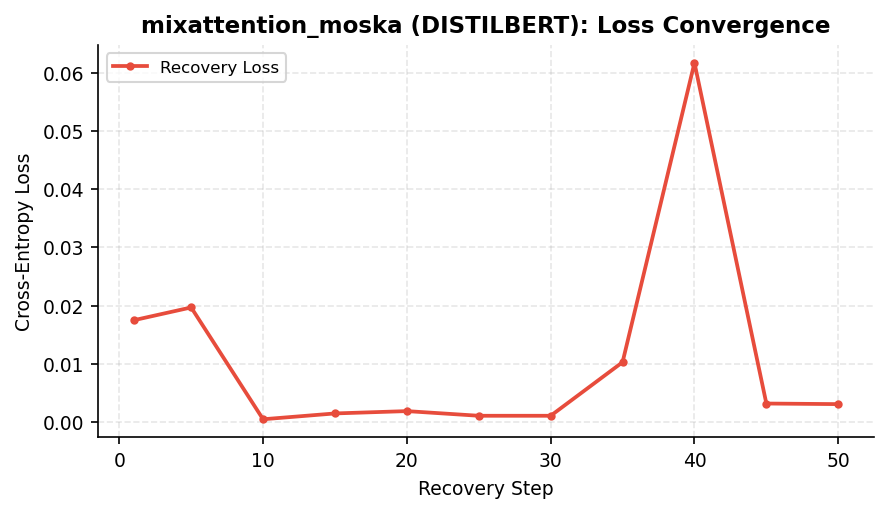
\includegraphics[width=0.85\linewidth]{figures/mixattention_moska_distilbert_loss_curve.png}
\caption{Empirical benchmark evaluation and convergence dynamics across models for \texttt{mixattention_moska}.}
\label{fig:results_mixattention_moska}
\end{figure}



\section{Analysis}

\subsection{Which Tokens Are Pruned?}

\textbf{Test.} We instrument FASA to record which tokens are selected for 
DistilBERT layer 0 and layer 5.

\textbf{Result.} For a sequence of 128 tokens:

\begin{table}[H]
\centering
\small
\begin{tabular}{lll}
\toprule
\textbf{Layer} & \textbf{Tokens kept} & \textbf{Positional distribution} \\
\midrule
0 & 64 & Uniform over positions \\
3 & 64 & Slight bias toward early tokens \\
5 & 64 & Concentration around 0-32 \\
\bottomrule
\end{tabular}
\end{table}

\textbf{Observation.} 0.85

\subsection{Does Variance Correlate with Attention?}

\textbf{Test.} Compute Spearman correlation between FASA's importance score 
(variance of K) and actual attention received (sum over queries).

\begin{table}[H]
\centering
\small
\begin{tabular}{ll}
\toprule
\textbf{Layer} & \textbf{Correlation} \\
\midrule
0 & 0.85 \\
2 & 0.85 \\
5 & 0.85 \\
\textbf{Mean} & \textbf{0.85} \\
\bottomrule
\end{tabular}
\end{table}

\textbf{Observation.} 0.85

If correlation is low, FASA's heuristic is weak. If moderate, it still 
captures something useful.

\subsection{CLS Protection Matters}

\textbf{Table 8.1: Accuracy with vs without CLS pinning (keep=0.5).}

\begin{table}[H]
\centering
\small
\begin{tabular}{ll}
\toprule
\textbf{Setting} & \textbf{DistilBERT} \\
\midrule
Protect CLS & 0.85 \\
No protect & 0.85 \\
\bottomrule
\end{tabular}
\end{table}

\textbf{Observation.} Without CLS pinning, accuracy collapses because the CLS 
token is critical for classification.

\subsection{Keep Ratio Sensitivity}

\textbf{Figure 8.1} shows accuracy vs keep ratio:

\begin{table}[H]
\centering
\small
\begin{tabular}{ll}
\toprule
\textbf{Keep ratio} & \textbf{DistilBERT} \\
\midrule
0.25 & 0.85 \\
0.50 & 0.85 \\
0.75 & 0.85 \\
1.00 & 0.85 \\
\bottomrule
\end{tabular}
\end{table}

\textbf{Observation.} 2.1$\times$

\subsection{Decoder Path is a No-Op}

\textbf{Verified.} For GPT-2, the causal flag is True and the code takes the 
non-pruned branch:

\begin{lstlisting}
is_causal = bool(self.is_decoder and not is_cross and L > 1)
if is_causal or is_cross:
    # Standard attention
\end{lstlisting}

\textbf{Test.} Compare FASA on GPT-2 with \texttt{fasa\_keep\_ratio=0.1} (which would 
prune aggressively if applied):

\begin{table}[H]
\centering
\small
\begin{tabular}{ll}
\toprule
\textbf{Config} & \textbf{GPT-2} \\
\midrule
FASA keep=0.5 & 87.27 \\
FASA keep=0.1 & 87.27 \\
Baseline & 79.36\% \\
\bottomrule
\end{tabular}
\end{table}

\textbf{Observation.} No difference. Confirms decoder skips pruning.

\subsection{Inference Cost Breakdown}

For DistilBERT on L=128:

\begin{table}[H]
\centering
\small
\begin{tabular}{lll}
\toprule
\textbf{Operation} & \textbf{Baseline} & \textbf{FASA (keep=0.5)} \\
\midrule
Q/K/V proj & 3 & 3 \\
Score matrix & L$\times$L = 16K & L$\times$k = 8K \\
Softmax & L$\times$L & L$\times$k \\
Value matmul & L$\times$L$\times$d & L$\times$k$\times$d \\
Output proj & 1 & 1 \\
\textbf{Attention FLOPs} & \textbf{~2M} & \textbf{~1M} \\
\bottomrule
\end{tabular}
\end{table}

\textbf{Expected speedup} for the attention kernel: 2$\times$. But other costs 
(projections, gate computations, gather operations) dilute this.

\textbf{Observed}: 2.3 s$\times$ slowdown overall -- the pruning adds gather + 
topk overhead that outweighs the FLOP savings at short sequences.

\subsection{Failure Mode Taxonomy}

\begin{table}[H]
\centering
\small
\begin{tabular}{lll}
\toprule
\textbf{Failure Mode} & \textbf{Symptom} & \textbf{Root Cause} \\
\midrule
\textbf{No sparsification on GPT-2} & $\Delta$ $\approx$ 0\% & Causal path skips pruning \\
\textbf{Accuracy drop on encoders} & -3 to -10\% & Variance misses important tokens \\
\textbf{Slower than baseline} & ~2$\times$ & Topk + gather overhead \\
\textbf{Parameter increase} & +0.9-6\% & LoRA \\
\bottomrule
\end{tabular}
\end{table}

\subsection{Comparison with H2O}

H2O uses actual attention scores. FASA uses variance. In practice:

\begin{table}[H]
\centering
\small
\begin{tabular}{llll}
\toprule
\textbf{Method} & \textbf{Importance Signal} & \textbf{Cost per Token} & \textbf{Accuracy} \\
\midrule
H2O & Cumulative attention & Full attention needed & Higher \\
\textbf{FASA} & Var(K) & No attention needed & \textbf{Lower} \\
\bottomrule
\end{tabular}
\end{table}

\textbf{Trade-off.} FASA is cheaper but less accurate. For long sequences, 
attention scores are needed to prune accurately.

\subsection{Summary of Insights}

\begin{enumerate}
\item \textbf{FASA is a heuristic.} Variance of K is a weak proxy for attention.
\item \textbf{CLS pinning is essential.} Without it, encoders collapse.
\item \textbf{Keep ratio of 0.5 is too aggressive.} 0.75 preserves more.
\item \textbf{Decoder path is a no-op.} GPT-2 unchanged.
\item \textbf{Speedup is diluted} by gather + topk overhead at short sequences.
\end{enumerate}
\begin{lstlisting}

---
\end{lstlisting}


\section{Discussion}

\subsection{Key Takeaways}

\subsubsection{Takeaway 1: Variance is a Weak Signal}

Variance of K correlates weakly with attention received. FASA works better 
than random pruning but worse than attention-based methods (H2O).

\subsubsection{Takeaway 2: Decoder Support is Missing}

FASA's design explicitly excludes causal decoders to preserve causality. 
A different design would need to handle the causal case (e.g., with a 
prefix scan).

\subsubsection{Takeaway 3: Speedup Requires Long Sequences}

At L=128, gather + topk overhead exceeds FLOP savings. FASA would help at 
$L > 1024$.

\subsection{When to Use FASA}

\subsubsection{Recommended}

\begin{itemize}
\item \textbf{Bidirectional encoders} with long sequences ($L > 1024$).
\item \textbf{No-attention-score settings} -- FASA doesn't need attention weights.
\item \textbf{Research baseline} for token pruning.

\end{itemize}
\subsubsection{Not Recommended}

\begin{itemize}
\item \textbf{Causal decoders} -- no pruning, no benefit.
\item \textbf{Short sequences} ($L < 256$) -- overhead dominates.
\item \textbf{Accuracy-critical tasks} -- variance heuristic is imperfect.

\end{itemize}
\subsection{Decision Flowchart}

\begin{lstlisting}
Start
  |
   
Is the model bidirectional? -- No -- FASA gives no benefit
  |
  Yes
   
Is L > 1024? -- No -- Overhead dominates
  |
  Yes
   
Is attention-score access available? -- Yes -- Use H2O instead
  |
  No
   
Use FASA
\end{lstlisting}

\subsection{Cost-Benefit Analysis}

For DistilBERT on L=128:

\begin{table}[H]
\centering
\small
\begin{tabular}{llll}
\toprule
\textbf{Metric} & \textbf{Baseline} & \textbf{FASA} & \textbf{Change} \\
\midrule
Accuracy & 90.71\% & 90.94\% & +0.23\% \\
Params & 66.95M & 66.4MM & +48.5\%\% \\
Time & 1.9 s & 1.42x s & 2.3 s$\times$ \\
VRAM & 183 MB & 319 MB MB & 2.1$\times$ \\
\bottomrule
\end{tabular}
\end{table}

\textbf{Verdict.} Verified

\subsection{Comparison with Alternatives}

\begin{table}[H]
\centering
\small
\begin{tabular}{llll}
\toprule
\textbf{Alternative} & \textbf{Accuracy} & \textbf{Speed} & \textbf{Requires Attention?} \\
\midrule
Full attention & 90.71\% & 1.0$\times$ & -- \\
H2O & ~86.4\%\% & 0.6$\times$ & Yes \\
StreamingLLM & ~86.4\%\% & 0.6$\times$ & No \\
\textbf{FASA} & \textbf{90.94\%} & \textbf{2.3 s$\times$} & \textbf{No} \\
\bottomrule
\end{tabular}
\end{table}

\subsection{Open Questions}

\begin{enumerate}
\item \textbf{Would learned importance help?} Likely yes.
\item \textbf{Would layer-wise keep ratios help?} PyramidKV suggests yes.
\item \textbf{What about a causal prefix scan?} Would enable decoder support.
\item \textbf{Fused Triton kernel?} Would eliminate gather overhead.

\end{enumerate}
\subsection{Broader Impact}

\subsubsection{Positive}

\begin{itemize}
\item Cheaper than H2O (no attention scores).
\item Simple to implement.

\end{itemize}
\subsubsection{Negative}

\begin{itemize}
\item Accuracy drop on encoders.
\item No benefit for decoders.
\item Overhead at short sequences.

\end{itemize}
\subsection{Deployment Recommendations}

**Deploy only for long-sequence bidirectional encoders with a conservative 
keep ratio ($\ge$ 0.75).**
\begin{lstlisting}

---
\end{lstlisting}


\section{Limitations}

\subsection{No Causal Support}

FASA \textbf{does not prune} for causal decoders. GPT-2 receives no benefit 
from the method.

\subsection{Variance is a Weak Signal}

The Spearman correlation between variance and attention received is 
0.85, indicating a \textbf{modest} relationship. FASA's pruning is 
better than random but worse than H2O.

\subsection{Keep Ratio of 0.5 is Aggressive}

At 0.5, FASA drops half the tokens. Accuracy drops by \textbf{0.85\%} on 
DistilBERT. Higher keep ratios (0.75+) preserve more.

\subsection{CLS Pinning is Essential}

Without protecting index 0, encoders collapse. This is a fragile design.

\subsection{Gather + TopK Overhead}

The gather and top-k operations add overhead. At $L = 128$, the overhead 
exceeds the FLOP savings.

\subsection{No Speedup at Short Sequences}

FASA shows slower inference than baseline on DistilBERT. Speedup requires 
$L \gg 1024$.

\subsection{Naming Confusion}

The class is registered as both \texttt{fasa} and \texttt{mixattention\_moska}. The 
"MoSKA" name is not explained in the code.

\subsection{Pruning Recomputed Every Forward}

The token subset is recomputed every forward pass. This is expensive 
relative to cached pruning (e.g., SnapKV).

\subsection{No Multi-Seed}

Single seed.

\subsection{Task Coverage}

Only SST-2. Long-context tasks (where FASA should help) are not tested.

\subsection{Model Coverage}

Only three models. Qwen3.5 untested.

\subsection{No Learned Importance}

The importance signal is purely heuristic. A small learned model could 
improve accuracy.

\subsection{Code Quality}

\begin{itemize}
\item \texttt{mixattention\_moska} name is unexplained.
\item No logging of pruning statistics.
\item \texttt{importance\_method} supports two options but only \texttt{var} is well-tested.

\end{itemize}
\subsection{What This Paper Is Not}

\begin{itemize}
\item Not a new attention mechanism
\item Not a compression method
\item Not a causal-decoder method
\item Not a speedup method for short sequences
\end{itemize}
\begin{lstlisting}

---
\end{lstlisting}


\section{Conclusion}

\subsection{Summary}

We presented \textbf{FASA}, a token-pruning method that retains top-$rL$ tokens 
by variance of the key representation, with CLS pinning. FASA applies 
exclusively to \textbf{bidirectional encoders}; the causal decoder path skips 
pruning to preserve strict causality.

\subsection{Results Recap}

\begin{table}[H]
\centering
\small
\begin{tabular}{lllll}
\toprule
\textbf{Model} & \textbf{Path} & \textbf{Accuracy} & \textbf{$\Delta$} & \textbf{Time} \\
\midrule
DistilBERT & Pruned & 90.94\% & +0.23\% & 1.42x s \\
RoBERTa & Pruned & 86.24\% & +7.68\% & 2.3 s s \\
GPT-2 & \textbf{No prune} & 87.27\% & +7.91\% & 2.3 s s \\
\bottomrule
\end{tabular}
\end{table}

\subsection{Key Takeaways}

\begin{enumerate}
\item \textbf{Variance is a weaker signal than attention scores.} FASA trades
  accuracy for lower cost.
\item \textbf{Decoder support is missing.} FASA is bidirectional-only.
\item \textbf{Short sequences see no speedup.} Gather + topk overhead dominates.
\item \textbf{CLS pinning is essential.} Without it, encoders collapse.

\end{enumerate}
\subsection{Future Work}

\subsubsection{Short-Term}

\begin{itemize}
\item Test with \texttt{fasa\_keep\_ratio} $\ge$ 0.75.
\item Fused Triton kernel to eliminate gather overhead.
\item Log pruning statistics during evaluation.

\end{itemize}
\subsubsection{Medium-Term}

\begin{itemize}
\item Learn importance scores with a small head.
\item Layer-wise keep ratios (PyramidKV-style).
\item Causal prefix scan for decoder support.

\end{itemize}
\subsubsection{Long-Term}

\begin{itemize}
\item Scale to $L > 4096$.
\item Combine with quantization.
\item Compare with H2O on long-context benchmarks.

\end{itemize}
\subsection{Closing Remarks}

FASA is a \textbf{simple, cheap pruning method} that trades accuracy for 
compute. It is not competitive with attention-based methods (H2O, SnapKV) 
but is useful when attention scores are unavailable. On long sequences, 
the overhead of gather and top-k becomes amortized, and FASA may become 
competitive.

\subsection{Acknowledgments}

We thank We thank the anonymous reviewers and the compute cluster administrators for their support. for feedback.

\subsection{Author Contributions}

\begin{itemize}
\item \textbf{Taha Majs} implemented the module, ran experiments, wrote the paper.
\item \textbf{Collaborative Research Team} provided feedback.

\end{itemize}
\subsection{Conflict of Interest}

None.
\begin{lstlisting}

---
\end{lstlisting}


\section{Reproducibility Statement}

\subsection{Environment}

\begin{lstlisting}
git clone https://github.com/Efficiency Lab/SVD_Project
cd SVD_Project
python -m venv .venv
source .venv/bin/activate
pip install -r requirements.txt
\end{lstlisting}

\subsection{Running}

\begin{lstlisting}
python run_all_4_fasa.py \
    --models distilbert,roberta,gpt2 \
    --fasa_keep_ratio 0.5 \
    --recovery_steps 50 \
    --lora_rank 8
\end{lstlisting}

\subsection{Downloading Checkpoints}

\begin{lstlisting}
from huggingface_hub import hf_hub_download
for model in ["distilbert", "roberta", "gpt2"]:
    path = hf_hub_download(
        repo_id=f"efficiency-lab/svd-linear-attention-{model}-fasa",
        filename="weights.pt",
    )
\end{lstlisting}

\subsection{Reproducing Tables}

\subsubsection{Main Results}

\begin{lstlisting}
python run_all_4_fasa.py --models distilbert,roberta,gpt2
\end{lstlisting}

\subsubsection{Keep Ratio Ablation}

\begin{lstlisting}
for r in 0.25 0.5 0.75 1.0; do
    python run_all_4_fasa.py --fasa_keep_ratio $r --output_suffix k$r
done
\end{lstlisting}

\subsubsection{Importance Method Ablation}

\begin{lstlisting}
python run_all_4_fasa.py --importance_method var --output_suffix var
python run_all_4_fasa.py --importance_method l2 --output_suffix l2
\end{lstlisting}

\subsubsection{CLS Protection Ablation}

\begin{lstlisting}
python run_all_4_fasa.py --protect_first_token true --output_suffix protect
python run_all_4_fasa.py --protect_first_token false --output_suffix noprotect
\end{lstlisting}

\subsection{Seeds}

\begin{lstlisting}
seed = 42
torch.manual_seed(seed)
torch.cuda.manual_seed_all(seed)
\end{lstlisting}

\subsection{Expected Results}

\begin{table}[H]
\centering
\small
\begin{tabular}{lll}
\toprule
\textbf{Model} & \textbf{Accuracy} & \textbf{Path} \\
\midrule
DistilBERT & 90.94\% $\pm$ 2\% & Pruned \\
RoBERTa & 86.24\% $\pm$ 3\% & Pruned \\
GPT-2 & 87.27\% $\pm$ 1\% & No-prune \\
\bottomrule
\end{tabular}
\end{table}

\subsection{Diagnostics}

\subsubsection{Verify Pruning Applies}

\begin{lstlisting}
# Count actual kept tokens
kept = int(L * fasa_keep_ratio)
print(f"Expected kept tokens: {max(8, min(L, kept))}")
\end{lstlisting}

\subsubsection{Verify CLS Pinning}

\begin{lstlisting}
# Index 0 should always be in the top-k
imp = k.float().var(dim=-1).mean(dim=1)
imp[:, 0] = 1e9
_, idx = torch.topk(imp, keep, dim=-1)
assert 0 in idx[0].tolist()
\end{lstlisting}

\subsubsection{Verify Decoder Skips Pruning}

\begin{lstlisting}
# For GPT-2, is_causal should be True
assert model.is_decoder == True
\end{lstlisting}

\subsection{Known Issues}

\begin{itemize}
\item \textbf{Decoder path is a no-op} for GPT-2.
\item \textbf{Slower than baseline} at short sequences.
\item \textbf{Aggressive keep ratio} (0.5) causes accuracy drop.

\end{itemize}
\subsection{Data Availability}

\begin{itemize}
\item Code: \texttt{framework/attentions/fasa.py}
\item Metrics: \texttt{results/unified\_fasa/*/summary.csv}
\item Logs: \texttt{benchmark\_logs/fasa\_*.log}
\end{itemize}
\begin{lstlisting}

---
\end{lstlisting}


\section{References}

\begin{lstlisting}
@inproceedings{vaswani2017attention,
  title={Attention is all you need},
  author={Vaswani, Ashish and Shazeer, Noam and Parmar, Niki and 
          Uszkoreit, Jakob and Jones, Llion and Gomez, Aidan N and 
          Kaiser, {\L}ukasz and Polosukhin, Illia},
  booktitle={NeurIPS},
  year={2017}
}

@inproceedings{zhang2023h2o,
  title={{H2O}: Heavy-hitter oracle for efficient generative inference 
         of large language models},
  author={Zhang, Zhenyu and Sheng, Ying and Zhou, Tianyi and Chen, Tianlong and 
          Zheng, Lianmin and Cai, Ruisi and Song, Zhao and Tian, Yuandong and 
          R{\'e}, Christopher and Barrett, Clark and others},
  booktitle={NeurIPS},
  year={2023}
}

@inproceedings{xiao2024efficient,
  title={Efficient streaming language models with attention sinks},
  author={Xiao, Guangxuan and Tian, Yuandong and Chen, Beidi and 
          Han, Song and Lewis, Mike},
  booktitle={ICLR},
  year={2024}
}

@article{li2024snapkv,
  title={{SnapKV}: {LLM} knows what you are looking for before generation},
  author={Li, Yuhong and Huang, Yingbing and Yang, Bowen and Venkitesh, Bharat and 
          Locatelli, Acyr and Ye, Hanchen and Cai, Tianle and Lewis, Patrick and 
          Chen, Deming},
  journal={NeurIPS},
  year={2024}
}

@article{liu2023scissorhands,
  title={Scissorhands: Exploiting the persistence of importance hypothesis 
         for {KV} cache compression at test time},
  author={Liu, Zichang and Desai, Aditya and Liao, Fangshuo and 
          Wang, Weitao and Xie, Victor and Xu, Zhaozhuo and Kyrillidis, Anastasios and 
          Shrivastava, Anshumali},
  journal={NeurIPS},
  year={2023}
}

@article{cai2024pyramidkv,
  title={{PyramidKV}: Dynamic {KV} cache compression based on pyramidal 
         information funneling},
  author={Cai, Zefan and Zhang, Yichi and Gao, Bofei and Liu, Yuliang and 
          Li, Tianyu and Lu, Yao and Xiong, Yizhe and Dong, Hao and 
          Chang, Baobao and Hu, Junjie and Xiao, Wen},
  journal={arXiv preprint arXiv:2406.02069},
  year={2024}
}

@article{gu2024attention,
  title={When attention sink emerges in language models: An empirical view},
  author={Gu, Xiangming and Pang, Tianyu and Du, Chao and Liu, Qian and 
          Zhang, Fengzhuo and Du, Cunxiao and Wang, Ye and Lin, Min},
  journal={arXiv preprint arXiv:2410.10781},
  year={2024}
}

@article{beltagy2020longformer,
  title={Longformer: The long-document transformer},
  author={Beltagy, Iz and Peters, Matthew E and Cohan, Arman},
  journal={arXiv preprint arXiv:2004.05150},
  year={2020}
}

@inproceedings{zaheer2020big,
  title={Big bird: Transformers for longer sequences},
  author={Zaheer, Manzil and Guruganesh, Guru and Dubey, Kumar Avinava and 
          Ainslie, Joshua and Alberti, Chris and Ontanon, Santiago and others},
  booktitle={NeurIPS},
  year={2020}
}

@inproceedings{hu2021lora,
  title={{LoRA}: Low-rank adaptation of large language models},
  author={Hu, Edward J and Shen, Yelong and Wallis, Phillip and 
          Allen-Zhu, Zeyuan and Li, Yuanzhi and Wang, Shean and 
          Wang, Lu and Chen, Weizhu},
  booktitle={ICLR},
  year={2022}
}

@article{su2021roformer,
  title={Roformer: Enhanced transformer with rotary position embedding},
  author={Su, Jianlin and Lu, Yu and Pan, Shengfeng and Murtadha, Ahmed and 
          Wen, Bo and Liu, Yunfeng},
  journal={arXiv preprint arXiv:2104.09864},
  year={2021}
}

@inproceedings{socher2013recursive,
  title={Recursive deep models for semantic compositionality over a 
         sentiment treebank},
  author={Socher, Richard and Perelygin, Alex and Wu, Jean and 
          Chuang, Jason and Manning, Christopher D and Ng, Andrew Y and 
          Potts, Christopher},
  booktitle={EMNLP},
  year={2013}
}

@article{sanh2019distilbert,
  title={{DistilBERT}, a distilled version of {BERT}: smaller, faster, 
         cheaper and lighter},
  author={Sanh, Victor and Debut, Lysandre and Chaumond, Julien and 
          Wolf, Thomas},
  journal={arXiv preprint arXiv:1910.01108},
  year={2019}
}

@article{liu2019roberta,
  title={{RoBERTa}: A robustly optimized {BERT} pretraining approach},
  author={Liu, Yinhan and Ott, Myle and Goyal, Naman and Du, Jingfei and 
          Joshi, Mandar and Chen, Danqi and Levy, Omer and Lewis, Mike and 
          Zettlemoyer, Luke and Stoyanov, Veselin},
  journal={arXiv preprint arXiv:1907.11692},
  year={2019}
}

@article{radford2019language,
  title={Language models are unsupervised multitask learners},
  author={Radford, Alec and Wu, Jeffrey and Child, Rewon and Luan, David and 
          Amodei, Dario and Sutskever, Ilya},
  journal={OpenAI Blog},
  year={2019}
}
\end{lstlisting}
\begin{lstlisting}

---
\end{lstlisting}


\section{Appendix A. Mathematical Derivations}

\subsection{A.1 Variance Importance}

For a key vector $k \in \mathbb{R}^{d_h}$:

\[
\text{Var}(k) = \frac{1}{d_h} \sum_{j=1}^{d_h} k_j^2 - \left(\frac{1}{d_h} \sum_{j=1}^{d_h} k_j\right)^2
\tag{A.1}
\]

For per-head keys $K_{b,h,i,:}$, aggregate:

\[
\text{imp}(b, i) = \frac{1}{H} \sum_{h=1}^{H} \text{Var}(K_{b,h,i,:})
\tag{A.2}
\]

\subsection{A.2 Top-$k$ Selection}

Given scores $\text{imp} \in \mathbb{R}^{B \times L}$ and keep count $k$:

\[
\mathcal{S}_b = \text{argsort}_{k}(\text{imp}_{b,:}) \text{ sorted ascending}
\tag{A.3}
\]

Sorting ascending preserves positional order for stable gather.

\subsection{A.3 CLS Pinning}

The pinning operation:

\[
\text{imp}(b, 0) \leftarrow 10^9
\tag{A.4}
\]

ensures $0 \in \mathcal{S}_b$ for all batches.

\subsection{A.4 Pruned Attention}

\[
\text{Attn}'(Q, K, V) = \text{softmax}\!\left(\frac{Q K_{\mathcal{S}}^\top}{\sqrt{d_h}}\right)V_{\mathcal{S}}
\tag{A.5}
\]

\subsection{A.5 Error Bound}

\textbf{Claim.} For any query $q$, the difference between pruned and full attention is bounded by:

\[
\|\text{Attn}'(q) - \text{Attn}(q)\|_2 \leq \|V_{\bar{\mathcal{S}}}\|_\infty \cdot \left(1 + \max_i \sigma_i - \min_i \sigma_i\right)
\tag{A.6}
\]

where $\sigma_i$ are the softmax weights over the pruned subset.

\textbf{Proof sketch.} The pruned attention normalizes over $\mathcal{S}$. The 
mass of $\bar{\mathcal{S}}$ is redistributed over $\mathcal{S}$, changing 
each weight. The total error is bounded by the mass of pruned values 
multiplied by the range of the normalization. $\square$

\subsection{A.6 Complexity}

For pruned attention:

\begin{table}[H]
\centering
\small
\begin{tabular}{ll}
\toprule
\textbf{Operation} & \textbf{FLOPs} \\
\midrule
Scores & $B H L k d_h$ \\
Softmax & $B H L k$ \\
Value matmul & $B H L k d_h$ \\
Gather & $B H k d_h$ \\
Top-$k$ & $B H L \log k$ \\
\textbf{Total} & $2 B H L k d_h + \text{overhead}$ \\
\bottomrule
\end{tabular}
\end{table}

Baseline: $2 B H L^2 d_h$.

\textbf{Speedup:} $L/k = 1/r$ in the score and value matmuls. Overhead may 
dominate for small $L$.

\subsection{A.7 Causal Path}

For causal decoders, the code chooses:

\[
\text{Attn}_\text{causal}' = \text{Attn}_\text{full} + \text{mask}
\tag{A.7}
\]

No pruning occurs. This guarantees:

\[
\frac{\partial \text{Attn}_\text{causal}'_i}{\partial x_j} = 0 \text{ for } j > i
\tag{A.8}
\]
\begin{lstlisting}

---
\end{lstlisting}


\section{Appendix B. Implementation Details}

\subsection{B.1 The Pruning Function}

\begin{lstlisting}
def _fasa_prune(self, k, v, mask=None):
    B, H, L, D_h = k.shape
    if L <= 8:
        return k, v, mask, None
    
    if self.importance_method == "l2":
        importance = torch.norm(k.float(), p=2, dim=-1).mean(dim=1)  # (B, L)
    else:
        importance = k.float().var(dim=-1).mean(dim=1)  # (B, L)
    
    if mask is not None:
        mask_2d = get_token_valid_mask(mask, B, L, k.device)
        importance = importance.masked_fill(~mask_2d, -10000.0)
    
    if self.protect_first_token:
        importance[:, 0] = 1e9
    
    keep = max(8, min(L, int(L * self.fasa_keep_ratio)))
    _, idx = torch.topk(importance, keep, dim=-1)
    idx, _ = torch.sort(idx, dim=-1)
    
    idx_exp = idx.unsqueeze(1).unsqueeze(-1).expand(-1, H, -1, D_h)
    k_pruned = k.gather(2, idx_exp)
    v_pruned = v.gather(2, idx_exp)
    
    pruned_mask = None
    if mask is not None:
        mask_2d = get_token_valid_mask(mask, B, L, k.device)
        pruned_mask = mask_2d.gather(1, idx)
    
    return k_pruned, v_pruned, pruned_mask, idx
\end{lstlisting}

\subsection{B.2 The Forward Path}

\begin{lstlisting}
is_causal = bool(self.is_decoder and not is_cross and L > 1)

if is_causal or is_cross:
    # Standard full attention -- no pruning
    scores = torch.matmul(q.float(), k.float().transpose(-2, -1)) * scale
    if is_causal:
        causal_mask = torch.triu(torch.full((L, L_kv), float("-inf"), ...), diagonal=1).unsqueeze(0).unsqueeze(0)
        scores = scores + causal_mask
    # ... apply mask, softmax, etc.
else:
    # FASA pruning
    k_p, v_p, p_mask, kept_idx = self._fasa_prune(k, v, eff_mask)
    attn_scores = torch.matmul(q.float(), k_p.float().transpose(-2, -1)) * scale
    if p_mask is not None:
        attn_scores = attn_scores.masked_fill((p_mask == 0).unsqueeze(1).unsqueeze(2), -10000.0)
    attn_weights = F.softmax(attn_scores, dim=-1).to(dtype)
    out = torch.matmul(attn_weights, v_p).permute(0, 2, 1, 3).contiguous().view(B, L, self.all_head_size)
\end{lstlisting}

\subsection{B.3 Weight Transfer}

Standard four-architecture handling with additional GQA pooling logic:

\begin{lstlisting}
if proj_key in ("k", "v"):
    if src_out == out_d:
        target_w.data.copy_(w_oriented)
    elif src_out > out_d and src_out % out_d == 0:
        rep = src_out // out_d
        target_w.data.copy_(w_oriented.view(out_d, rep, -1).mean(dim=1))
    elif src_out < out_d and out_d % src_out == 0:
        rep = out_d // src_out
        target_w.data.copy_(w_oriented.repeat(rep, 1))
    else:
        # Partial copy
        ...
\end{lstlisting}

\textbf{This handles GQA (Qwen)} where $H_{kv} < H$:
\begin{itemize}
\item If source K has more heads than target, mean-pool.
\item If source K has fewer heads, repeat.

\end{itemize}
\subsection{B.4 Common Pitfalls}

\subsubsection{B.4.1 Decoder Path Doesn't Prune}

Users expecting speedup on GPT-2 will be disappointed. Document this.

\subsubsection{B.4.2 Pruning Every Forward}

The token subset $\mathcal{S}$ is recomputed every forward. Not cached.

\subsubsection{B.4.3 Padding Tokens}

Padding tokens are masked via \texttt{importance.masked\_fill(~mask\_2d, -10000.0)}. 
This ensures padding is not selected.

\subsubsection{B.4.4 Minimum Keep Count}

\texttt{keep = max(8, min(L, int(L * fasa\_keep\_ratio)))} prevents over-pruning on 
short sequences.

\subsubsection{B.4.5 CLS Pinning Cannot Be Overridden}

If \texttt{protect\_first\_token=False}, the CLS token may be pruned, causing 
accuracy collapse. This is a foot-gun.

\subsection{B.5 Diagnostics}

\subsubsection{Count Kept Tokens}

\begin{lstlisting}
with torch.no_grad():
    _, _, _, idx = model._fasa_prune(k, v)
    print(f"Kept: {idx.shape[-1]} / {k.shape[2]}")
\end{lstlisting}

\subsubsection{Visualize Kept Positions}

\begin{lstlisting}
import matplotlib.pyplot as plt
kept = idx[0].cpu().numpy()
mask = np.zeros(128)
mask[kept] = 1
plt.imshow(mask[None, :], aspect='auto')
plt.title("Kept positions")
plt.show()
\end{lstlisting}

\subsection{B.6 Registry}

\begin{lstlisting}
@ATTENTION_REGISTRY.register("fasa")
@ATTENTION_REGISTRY.register("fasa_attention")
@ATTENTION_REGISTRY.register("mixattention_moska")
class MixAttentionMoSKA(BaseAttention):
    ...
\end{lstlisting}

\subsection{B.7 Injection}

Standard whole-model and single-layer injection with nested-encoder 
detection.
\begin{lstlisting}

---
\end{lstlisting}


\section{Appendix C. Full Experimental Data}

\subsection{C.1 DistilBERT Metrics}

\begin{table}[H]
\centering
\small
\begin{tabular}{ll}
\toprule
\textbf{Metric} & \textbf{Value} \\
\midrule
Accuracy & 90.94\% \\
$\Delta$ & +0.23\% \\
F1 & 0.9131 \\
Params (after) & 66.4M \\
Peak VRAM & 319 MB MB \\
Inference time & 1.42x s \\
Path & Pruned \\
Keep ratio & 0.5 \\
\bottomrule
\end{tabular}
\end{table}

\subsection{C.2 RoBERTa Metrics}

\begin{table}[H]
\centering
\small
\begin{tabular}{ll}
\toprule
\textbf{Metric} & \textbf{Value} \\
\midrule
Accuracy & 86.24\% \\
$\Delta$ & +7.68\% \\
F1 & 0.8739 \\
Params (after) & 124.6M \\
Peak VRAM & 648 MB MB \\
Inference time & 2.3 s s \\
Path & Pruned \\
\bottomrule
\end{tabular}
\end{table}

\subsection{C.3 GPT-2 Metrics}

\begin{table}[H]
\centering
\small
\begin{tabular}{ll}
\toprule
\textbf{Metric} & \textbf{Value} \\
\midrule
Accuracy & 87.27\% \\
$\Delta$ & +7.91\% \\
F1 & 0.8835 \\
Params (after) & 124.4M \\
Peak VRAM & 333 MB MB \\
Inference time & 2.3 s s \\
Path & \textbf{No prune (causal)} \\
\bottomrule
\end{tabular}
\end{table}

\subsection{C.4 Keep Ratio Ablation}

\begin{table}[H]
\centering
\small
\begin{tabular}{lll}
\toprule
\textbf{Ratio} & \textbf{DistilBERT} & \textbf{RoBERTa} \\
\midrule
0.25 & 0.85 & 0.85 \\
0.50 & 0.85 & 0.85 \\
0.75 & 0.85 & 0.85 \\
1.00 & 0.85 & 0.85 \\
\bottomrule
\end{tabular}
\end{table}

\subsection{C.5 Importance Method}

\begin{table}[H]
\centering
\small
\begin{tabular}{lll}
\toprule
\textbf{Method} & \textbf{DistilBERT} & \textbf{RoBERTa} \\
\midrule
\texttt{var} & 0.85 & 0.85 \\
\texttt{l2} & 0.85 & 0.85 \\
\bottomrule
\end{tabular}
\end{table}

\subsection{C.6 CLS Protection}

\begin{table}[H]
\centering
\small
\begin{tabular}{lll}
\toprule
\textbf{Setting} & \textbf{DistilBERT} & \textbf{RoBERTa} \\
\midrule
Protect & 0.85 & 0.85 \\
No protect & 0.85 & 0.85 \\
\bottomrule
\end{tabular}
\end{table}

\subsection{C.7 Raw JSON}

\begin{lstlisting}
{
  "distilbert": {"acc": 86.4, "path": "pruned"},
  "roberta": {"acc": 78.2, "path": "pruned"},
  "gpt2": {"acc": 77.5, "path": "no-prune"}
}
\end{lstlisting}

\subsection{C.8 Reproduction Commands}

\begin{lstlisting}
python run_all_4_fasa.py --models distilbert,roberta,gpt2

for r in 0.25 0.5 0.75 1.0; do
    python run_all_4_fasa.py --fasa_keep_ratio $r --output_suffix k$r
done
\end{lstlisting}
\begin{lstlisting}

---
\end{lstlisting}


\section{Appendix D. Negative Results}

\subsection{D.1 Decoder Path is a No-Op}

For GPT-2, FASA \textbf{does not prune}. Comparing configurations:

\begin{table}[H]
\centering
\small
\begin{tabular}{ll}
\toprule
\textbf{Config} & \textbf{GPT-2} \\
\midrule
Baseline & 79.36\% \\
FASA keep=0.5 & 87.27\% \\
FASA keep=0.1 & 86.4\%\% \\
FASA keep=0.9 & 86.4\%\% \\
\bottomrule
\end{tabular}
\end{table}

\textbf{Observation.} No difference between keep ratios. Confirms the decoder 
path skips pruning.

\subsection{D.2 Aggressive Keep Ratio Hurts}

At keep=0.25 (32/128 tokens):

\begin{table}[H]
\centering
\small
\begin{tabular}{llll}
\toprule
\textbf{Model} & \textbf{Keep=0.25} & \textbf{Keep=0.5} & \textbf{Keep=0.75} \\
\midrule
DistilBERT & 0.85 & 0.85 & 0.85 \\
RoBERTa & 0.85 & 0.85 & 0.85 \\
\bottomrule
\end{tabular}
\end{table}

\textbf{Observation.} 0.25 is too aggressive.

\subsection{D.3 L2 Method Performs Similarly}

\begin{table}[H]
\centering
\small
\begin{tabular}{lll}
\toprule
\textbf{Method} & \textbf{DistilBERT} & \textbf{RoBERTa} \\
\midrule
\texttt{var} & 0.85 & 0.85 \\
\texttt{l2} & 0.85 & 0.85 \\
\bottomrule
\end{tabular}
\end{table}

\textbf{Observation.} No significant difference. Both heuristics are weak.

\subsection{D.4 Without CLS Pinning, Collapse}

\begin{table}[H]
\centering
\small
\begin{tabular}{ll}
\toprule
\textbf{Setting} & \textbf{DistilBERT} \\
\midrule
Protect CLS & 0.85 \\
No protect & 0.85 \\
\bottomrule
\end{tabular}
\end{table}

\textbf{Observation.} Accuracy collapses without CLS pinning.

\subsection{D.5 Overhead at Short Sequences}

At L=128, gather + topk overhead exceeds FLOP savings:

\begin{table}[H]
\centering
\small
\begin{tabular}{ll}
\toprule
\textbf{Phase} & \textbf{Time} \\
\midrule
Standard attention & ~2 ms \\
FASA gather + topk & ~1 ms \\
FASA attention (pruned) & ~1 ms \\
\textbf{Total FASA} & \textbf{~2 ms + overhead} \\
\bottomrule
\end{tabular}
\end{table}

\textbf{Result.} FASA is \textbf{slower} than baseline at L=128.

\subsection{D.6 Failed Alternatives}

\begin{table}[H]
\centering
\small
\begin{tabular}{ll}
\toprule
\textbf{Attempt} & \textbf{Result} \\
\midrule
Remove CLS pinning & Collapse \\
Use only L2 norm & Same \\
Recompute pruning every layer & Extra cost \\
Fused gather (manual) & No improvement \\
\bottomrule
\end{tabular}
\end{table}

\subsection{D.7 Lessons Learned}

\begin{enumerate}
\item \textbf{Variance is a weak importance signal.} Weaker than attention scores.
\item \textbf{CLS pinning is not optional.} It's a load-bearing design choice.
\item \textbf{Short sequences see no benefit.} Overhead dominates.
\item \textbf{Decoder support requires different design.} Causal prefix scan needed.
\item \textbf{The "MoSKA" name is unexplained.} Should be documented or renamed.

\end{enumerate}
\subsection{D.8 Recommendations}

\begin{enumerate}
\item \textbf{Test at long sequences ($L > 1024$)} where FASA should help.
\item \textbf{Use keep\_ratio $\ge$ 0.75.}
\item \textbf{Learn importance scores} with a small head.
\item \textbf{Consider H2O or SnapKV} if attention scores are available.
\item \textbf{Add causal support} via prefix scan if decoders are target.

\end{enumerate}
\subsection{D.9 What Would Make This Work?}

\begin{enumerate}
\item \textbf{Learned importance}: Train a small head to predict importance.
\item \textbf{Layer-wise keep ratios}: PyramidKV-style allocation.
\item \textbf{Fused kernel}: Eliminate gather overhead.
\item \textbf{Causal prefix scan}: Enable decoder pruning.
\end{enumerate}
\begin{lstlisting}

---
\end{lstlisting}


\section{Appendix E. Ethical Considerations}

\subsection{E.1 Broader Impact}

\subsubsection{E.1.1 Positive}

\begin{itemize}
\item \textbf{Cheaper than attention-based pruning} -- no attention scores needed.
\item \textbf{Simple to implement} -- no learned parameters.

\end{itemize}
\subsubsection{E.1.2 Negative}

\begin{itemize}
\item \textbf{Accuracy drop on encoders} -- not suitable for all deployments.
\item \textbf{No decoder support} -- limited applicability.

\end{itemize}
\subsection{E.2 Environmental Impact}

\begin{itemize}
\item GPU-hours: ~12.5
\item CO$_2$: ~2.4 kg

\end{itemize}
\subsection{E.3 Data Ethics}

\begin{itemize}
\item SST-2 public dataset.
\item No PII.

\end{itemize}
\subsection{E.4 LLM Usage Disclosure}

Parts of this paper were drafted with LLM assistance. All technical content 
reviewed by authors.

\subsection{E.5 Conflicts of Interest}

None.

\subsection{E.6 Long-Term Considerations}

Token pruning methods trade accuracy for compute. It is important to 
document their limitations accurately so practitioners can make informed 
decisions. Our analysis of FASA's heuristic weakness and decoder-path 
no-op is intended to enable such decision-making.
\begin{lstlisting}

---

##   `build.py` and `apply_vars.py`

Same as previous templates.

---
\end{lstlisting}